% Converted from DOCX to an academic-style LaTeX article.
% Source file: PEPSY_core_paper_1_political_solidarity_europe_20260613 1100 (2).docx
\documentclass[12pt]{article}

\usepackage[a4paper,margin=1in]{geometry}
\usepackage[T1]{fontenc}
\usepackage[utf8]{inputenc}
\usepackage{textcomp}
\usepackage{lmodern}
\usepackage{microtype}
\usepackage{setspace}
\usepackage{amsmath,amssymb}
\usepackage{xcolor}
\usepackage{graphicx}
\usepackage{booktabs,longtable,array,calc}
\usepackage{caption}
\usepackage{etoolbox}
\usepackage{footnote}
\usepackage{newunicodechar}
\usepackage{xurl}
\usepackage[hidelinks]{hyperref}
\usepackage{bookmark}

\onehalfspacing
\setcounter{secnumdepth}{3}
\setcounter{tocdepth}{2}
\setlength{\parindent}{1.5em}
\setlength{\parskip}{0pt}
\setlength{\emergencystretch}{3em}
\urlstyle{same}
\captionsetup{font=small,labelfont=bf}

\makeatletter
\patchcmd\longtable{\par}{\if@noskipsec\mbox{}\fi\par}{}{}
\makeatother
\makesavenoteenv{longtable}
\providecommand{\tightlist}{\setlength{\itemsep}{0pt}\setlength{\parskip}{0pt}}
\newunicodechar{β}{\ensuremath{\beta}}

\title{What Explains Political Solidarity across Europe?\\
\large Novel Comparative Survey Evidence from Seven European Countries in 2026}
\author{Achim Goerres\thanks{University of Duisburg-Essen. \url{https://www.achimgoerres.de}} \and
Philipp Chapkovski\thanks{University of Duisburg-Essen. \url{https://chapkovski.github.io/}} \and
Jakob Eicheler\thanks{University of Duisburg-Essen. \url{https://www.jakob-eicheler.eu}} \and
Philipp Kemper\thanks{University of Duisburg-Essen. \url{https://philippckemper.de}}}
\date{Version: 13 June 2026}

\begin{document}
\maketitle

\begin{abstract}
European democracies increasingly rely on citizen support for costly public redistribution, from welfare-state reform to responses to migration, pandemics, war, and demographic change. This paper asks what explains political solidarity, understood as citizens' willingness to support public redistribution that benefits others. We develop a multilevel framework in which solidarity is shaped by individual foundations, social norms and state legitimacy, and objective regional and country contexts.

We test this framework using a new probability-based survey of 8,066 respondents in seven European countries in 2026, linked to regional and national indicators of governance, public-service quality, and economic context. We find substantial cross-national variation in political solidarity, broadly consistent with welfare-regime expectations, although the small number of country cases makes this evidence descriptive rather than a formal macro-level test.

The strongest evidence points to ideology and perceived state legitimacy. Respondents on the right are less supportive of political solidarity, while respondents who trust other people and institutions, perceive stronger contribution norms, and evaluate public services more positively are more willing to support redistribution for others. Perceived capacity to contribute and objective need or risk are also positively associated with solidarity. By contrast, objective socioeconomic resources, perceived personal risk, regional public-service quality, and relative regional income are not robust predictors in the full models. Overall, political solidarity appears to depend less on material position alone than on whether citizens regard the social and institutional environment as trustworthy, fair, and effective.
\end{abstract}

\noindent\textbf{Keywords:} political solidarity; redistribution; welfare state; Europe; survey evidence; public services

\vspace{1em}
\noindent\textbf{Funding and acknowledgements:} This paper is part of the POLITSOLID project funded by an ERC Consolidator Grant to the first-named author. Concept of the paper: all; survey development: AG (lead), PC, JE, PK; theory work: AG, PC; survey field management: JE; pilot analysis: PC, PK; statistical analysis: PC; first draft: AG, PC; final draft: all. Project information: \url{https://bit.ly/politsolid}.

\newpage
\section{\texorpdfstring{Introduction: political solidarity among
citizens in times of crises}{Introduction: political solidarity among citizens in times of crises }}\label{introduction-political-solidarity-among-citizens-in-times-of-crises}

Present-day democratic Europe seems to depend heavily on political
solidarity among its citizens, perhaps more visibly than at any point in
recent decades. In the financial crisis 2007-8, European Union countries
had to bail out other countries close to defaulting. In the years
2015-16, European citizens faced a large influx of humanitarian refugees
from war-torn Syria who had to be integrated into their societies. In
2020-22, Covid-19 required collective burden-sharing in vaccine
procurement, public-health restrictions, and emergency support. Since
2022, the war in Ukraine has triggered citizens' support for Ukrainian
refugees and for humanitarian and military aid to the Ukraine.

The literature on political solidarity is thereby dealing with very
different concepts of solidarity, from the normative to the empirical.
This empirical paper is about the citizens of Europe and about their
willingness to support other people by means of public redistribution
that is costly to themselves. \textbf{What explains general political
solidarity among citizens of Europe?}

Understanding the conditions of individual political solidarity is
relevant for two reasons. The demands for political solidarity may
become even higher in the next few years. For instance, a Russian attack
on further European countries may trigger the need for military,
citizen-supported alliance. Or, increasing negative climate change
consequences may necessitate the need for more state-led provisions and
citizen support. Moreover, European welfare states may have reached the
limits of sustainability. Due to population ageing and regionally
concentrated population decline, reforms to the welfare state, including
scaling back and re-financing state structures may test the limits of
political solidarity.

We test a multilevel model of political solidarity that combines
individual foundations, social norms and state legitimacy, and objective
regional and country contexts. As a first micro-level component, people
grow up and learn a certain level of political solidarity. This
unconditional political solidarity is deeply rooted in people' heads and
unlikely to change in the short term. Secondly, people are driven by
their own capacity to contribute. Solidarity is a function of short-term
ability to stand in for others. Thirdly, people watch out for themselves
when they strategically show political solidarity that can ultimately
benefit themselves. Then, turning towards the meso-level, people make
use of three kinds of perceptions -- about how the state is performing,
about how other contributors in the solidarity system are behaving and
about the beneficiaries of their political solidarity. At the macro
level, welfare-state institutions and fiscal capacity provide broader
contexts in which political solidarity is formed.

The data that we use are a novel comparative survey for seven European
countries: Croatia, France, Germany (East and West), Italy, Poland,
Spain and Sweden, collected in March and April 2026. They constitute a
broad set of welfare state institutional set-ups, historical pathways of
statecraft and levels of governance quality. The national samples are
randomly drawn from the resident adult population that allows
statistical inference about national populations, regional populations
and social groups. The data is augmented with contextual data about
regions and nations, thus allowing to test whether the subjective
perceptions of people are reflective of the objective state of the
world.

Our contribution is twofold. We analytically describe the levels of
political solidarity across nations, regions and social groups with
improved survey indicators in the year 2026. Furthermore, we
comprehensively test the multi-level model and reveal its most relevant
parts. Most importantly, we find that political solidarity is strongly
associated with ideology, social trust, institutional trust,
contribution norms, and evaluations of public services. By contrast,
objective socioeconomic resources and regional context play a less
consistent direct role once these perceptions are taken into account.

Why are people politically solidary? Our results point to five answers,
with unequal empirical support: people are more solidary when their
ideology favours redistribution, when they feel able to contribute, when
they have some exposure to social risks, when they believe others
contribute fairly, and when they trust institutions and public services
to deliver.

\section{Theoretical framework: a model of political
solidarity}\label{theoretical-framework-a-model-of-political-solidarity}

Political solidarity, defined as the willingness of citizens to support
welfare state policies that benefits others, is a product of causal
mechanisms at the macro, meso, and micro levels. At each level, both
objective conditions and subjective perceptions play a role, and their
intersection determines how strongly individuals support collective
welfare provisions. This section outlines a theoretical framework of
these factors, from individual predispositions and social norms to the
broader welfare state context. We make use of a political life cycle
model that integrates perspectives from early political socialization,
current socio-economic and institutional context. Figure 1 displays our
model that we want to test in this paper.

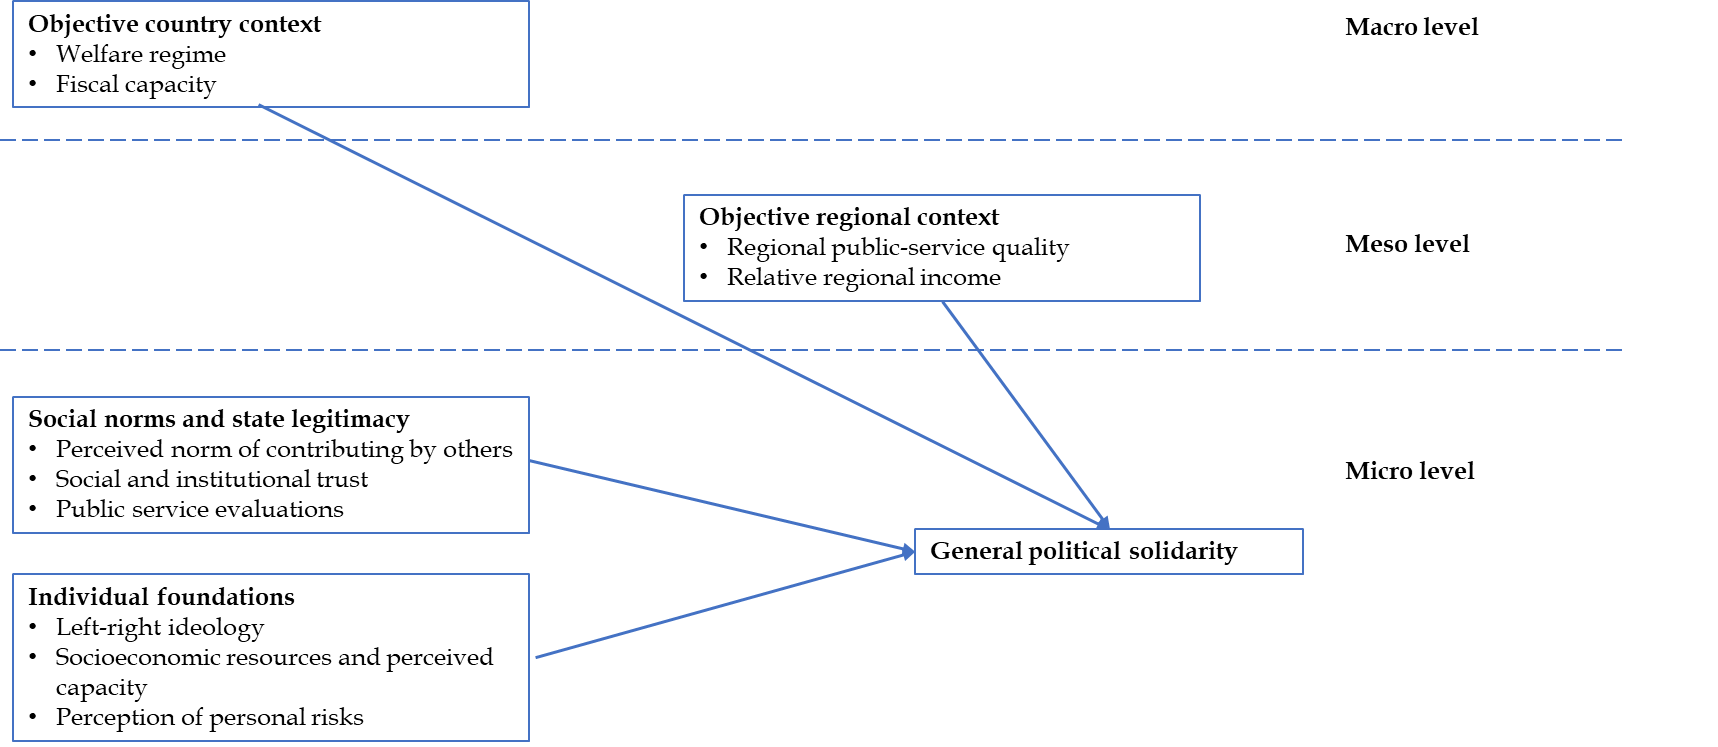
\includegraphics[width=6.26042in,height=2.71875in]{media/image1.png}

Figure 1: Our causal model of general political solidarity

\subsection{Micro-Level factors: ideology, resources, norms and state
legitimacy}\label{micro-level-factors-ideology-resources-norms-and-state-legitimacy}

\subsubsection{Political ideology and
resources}\label{political-ideology-and-resources}

At the \textbf{micro} level, an individual's own characteristics such as
their ideological values, material resources, and personal risks, have a
direct bearing on their support for political solidarity. Key
micro-level determinants include:

\textbf{Left-right ideology:} early in life, people are socialized into
an ideological predisposition and values. This early anchoring has
effects on their willingness to act in a politically solidary manner
towards others (Goerres and Eicheler 2025). An individual's ideological
leanings strongly influence their stance on welfare and solidarity.
Those with left-wing or egalitarian ideologies typically hold values of
social equality and collective responsibility, leading them to support
expansive welfare programs. In contrast, right-wing or economically
conservative individuals emphasize self-reliance, market solutions, and
limited government intervention, yielding more skepticism toward
redistribution (Feldman and Steenbergen 2001). This pattern is
well-documented across democracies: \emph{left-identifying citizens
consistently express higher support for the welfare state} (Roosma, van
Oorschot, and Gelissen 2014), whereas conservatives tend to endorse more
restrictive notions of solidarity (preferring, for example, that aid be
given only to the most ``deserving'' and favoring lower taxation) (Van
Der Waal, De Koster, and Van Oorschot 2013). These ideological
differences often persist even when controlling for income or personal
benefit.

\textbf{Socioeconomic resources:} In standard models of attitudes
towards the welfare state, material self-interest is regularly put
forward. People support policies that they benefit from (Baute and
Bellani 2025) or expect to benefit from in the future (Enggist,
Häusermann, and Pinggera 2022).; and people withdraw support from
policies that they only have to pay for but do not benefit from. In this
study, we are confronting respondents with the question for support for
policies of redistribution that others benefit from. Here are two
competing expectations about income. One might argue that richer
individuals show more political solidarity because they enjoy the
feeling of glow of doing something good for others, a mechanism that is
known from studies on philanthropy, or because they want stability in
the political system. Or, quite to the contrary, they show less
political solidarity because egoism makes them believe that in such a
system they are always least likely to benefit.

It is not only objective wealth that matters, but also subjective
perceptions of economic security. For example, an individual's
\emph{perceived capacity} to contribute (do they feel relatively
well-off or financially strained?) can modify their support for paying
into solidarity programs (Häusermann, Kurer, and Schwander 2016).
Someone who is objectively middle-class but feels financially insecure
or fears falling behind may be more supportive of welfare viewing it as
insurance (Rehm 2011). Subjective social status and feelings of economic
anxiety can therefore lead to variations that pure income rank would not
predict (Gimpelson and Treisman 2018).

In this study, we deliberately ask people for their support for public
redistribution that benefits other people, not themselves. By design, we
prime respondents that this is not about public programmes that they can
benefit directly. The income and perceived capacity can also be expected
to have positive effects. People may want to support such redistribution
to give stability to the system - like companies that mainly want a
stable system rather than a particular party in power. People with
higher incomes also may seek the glow of doing good for others. Many
studies of charitable donations (Elis, Mayer, Goerres 2024) actually
show that high-income individuals and those who have a positive outlook
on their personal income are most willing to donate to others.

People are also not atomised individuals without contacts to others. For
instance, in families, people are socially connected to individuals of
other age groups (one's children or parents)\\
It should be noted that these individual-level factors often interact in
complex ways. Ideology can moderate how one's income influences their
attitude (Cavaillé 2023). A wealthy social democrat may still support
redistribution strongly, while a poor person with conservative values
might oppose some welfare programs despite personally benefiting
(Armingeon and Weisstanner 2022). Likewise, personal experience with
hardship might soften ideological opposition (e.g., a fiscally
conservative person might become more supportive of welfare after
experiencing unemployment) (Harrs and Sterba 2023). Put simply, those
with higher incomes have more money to give but less reason to rely on
welfare, and those with lower incomes have more need but less ability to
finance it. This creates a potential conflict between contributors and
beneficiaries at the individual level. Many modern welfare states
resolve this by instituting universality (so that contributors also
benefit) or by fostering normative solidarity (convincing the well-off
to support the needy out of moral duty or enlightened self-interest).
The net effect on a person's support for solidarity depends on how they
balance self-interest and altruism. Specifically, on how policies affect
their own finances against their values and willingness to help others.
Political solidarity is highest when these factors align, for example,
when a person both needs assistance and ideologically believes in
egalitarianism. When they conflict (high need but strong belief in
self-reliance, or low need but strong egalitarian conviction) either
factor might prevail.

\subsubsection{Social norms and state
legitimacy}\label{social-norms-and-state-legitimacy}

A crucial intervening layer consists of social norms and perceptions of
``otherness.'' Societies can differ in the informal norms that govern
solidarity, essentially, shared expectations about whether fellow
citizens merit help and whether others are doing their part. These
normative perceptions create a \emph{social norm loop} that can
reinforce or undermine political solidarity (Bicchieri 2009).

One key element is generalized social trust: the belief that most other
people are honest and cooperative. High trust serves as a lubricant for
solidarity: if people assume others are not trying to cheat the system
and would likewise support them in need, they are more willing to pay
into collective welfare (Habibov, Cheung, and Auchynnikava 2017; Jensen
and Svendsen 2011). When social mistrust is rampant, people
\emph{``become less likely to feel solidarity with others outside their
own in-group''}, assuming that \emph{``few would voluntarily choose to
help them in their hour of need''} (Rothstein 2011, 96--98). In such a
low-trust climate, citizens doubt that others will reciprocate or that
beneficiaries are truly deserving, which leads to withdrawal of support
for expansive welfare. This dynamic illustrates how \textbf{beliefs
about others' contributions} condition one's own. If a person believes
that their peers widely support and contribute to solidarity (for
instance, that most people honestly pay their taxes and endorse helping
the vulnerable), that person is more inclined to do the same, sustaining
a high-solidarity equilibrium. On the other hand, if the belief spreads
that others are shirking (by not paying taxes, abusing benefits, or
opposing welfare) it can trigger a downward spiral of cynicism and
diminished support.

Finally, there is also the belief in the state's capacity to deliver. If
citizens are not satisfied with the way the state delivers, they may
question whether to be willing to pay into such a system (Levi 1997;
Rothstein 2021).

\subsection{Meso-level factors: Governance quality and regional
context}\label{meso-level-factors-governance-quality-and-regional-context}

At the \textbf{meso} level, two key contextual factors shape both
objective policy outcomes and citizens' perceptions: (1) the quality of
governance (including bureaucratic integrity and effectiveness), and (2)
the regional economic context within a country (Charron, Dijkstra, and
Lapuente 2013). These factors link national structures to everyday life
and shape how people see and practice solidarity.

Quality of governance, measured as the impartiality, efficiency, and
fairness of institutions, has a profound impact on political solidarity.
When public agencies implement welfare policies competently and fairly,
citizens are more willing to finance and support those policies.
Empirical studies confirm that \emph{``people who perceive public
institutions to be fair and efficient are more inclined to support
extensive welfare policies and provide resources for them''} (Svallfors
2013, p. 364). In a comparative survey of 29 European countries,
perceived high-quality government was associated with stronger support
for taxes and social spending, even after accounting for other factors
(Svallfors 2013). Good governance strengthens the link between
egalitarian beliefs and pro-welfare attitudes by assuring citizens that
solidarity will be implemented fairly (Kulin 2011). Recent micro-level
evidence shows that high-quality government does not simply raise
average support for redistribution but structures the income and
fairness divide itself: in countries with better government quality,
both income and unfairness perceptions become stronger predictors of
redistribution preferences (Ahrens 2024). In societies where corruption
is low and bureaucratic integrity high, egalitarian-minded individuals
are especially likely to demand robust social spending (Rothstein and
Uslaner 2005). The logic is intuitive: effective governance assures
citizens that their solidarity (e.g. tax contributions) will not be
siphoned off by corruption or wasted on inefficiency. According to Bo
Rothstein's theory, trustworthy and impartial institutions create a
foundation of social trust, making collective action feasible. By
contrast, in poorly governed settings, corruption and arbitrariness
corrode that trust. Studies have found that \emph{perceptions of
corruption can ``erode social solidarity,'' making citizens less willing
to cooperate or help those outside their own in-group} (Malmberg 2022).

Regional economic position is another meso-level factor that conditions
solidarity, especially in economically diverse countries. Within a
nation, regions often differ in prosperity, unemployment levels, and net
contribution to the national budget. People in wealthier regions usually
see themselves as net contributors to redistribution. Because of that,
they may be more skeptical of national solidarity programs that transfer
resources to other areas. In contrast, people in poorer regions who tend
to benefit from such transfers often show stronger support for
redistribution (Beramendi 2007). The territorial structure of inequality
influences preferences over fiscal policy centralization (Beramendi
2012). Where inter-regional income gaps are large, people's support for
solidarity can become fragmented along regional lines. Two mechanisms
are at play: \emph{``differences in the demand for redistribution
associated with interregional income differences, and differences in the
demand for social insurance associated with the incidence of labor
market risks''} (Beramendi 2007). Regional inequalities turn objective
economic differences into subjective judgments about who deserves help
(Gniza and Wrede 2024). For example, a taxpayer in a booming
metropolitan region might resent funding welfare programs perceived to
mainly assist other regions, unless a sense of national solidarity
prevails. On the flip side, a person in a depressed region might
perceive national solidarity as a lifeline and view opposition to it as
coming from unsympathetic ``others'' in wealthier areas. Regional
context thus shapes whether solidarity is seen as a unifying national
project or a zero-sum geographic transfer.

It is important to note that macro and meso factors also influence
subjective perceptions of the system's performance and fairness.
Objective indicators like GDP growth, unemployment rate, or inequality
level will affect whether individuals feel the country is ``doing well''
or if the economic system is just. Likewise, governance quality is
mirrored in public perceptions of bureaucratic fairness. These
perceptions, for example, whether ``things are going in the right
direction'' nationally, or whether officials are honest, feed into
support for solidarity policies. Thus, the meso context (quality of
government and regional economic standing) both directly affects
political solidarity (through actual policy performance and distributive
impacts) and indirectly affects it via perceptions of legitimacy and
fairness.

\subsection{Macro-level Factors: Welfare state regimes and fiscal
capacity}\label{macro-level-factors-welfare-state-regimes-and-fiscal-capacity}

At the societal \textbf{macro} level, the nature of the welfare state
and the state's fiscal capacity set the stage for political solidarity.
Different welfare state regimes embody distinct norms of solidarity.
Esping-Andersen's typology identifies, for example, liberal welfare
regimes that offer only modest, means-tested assistance targeted to the
poor often with strict, stigmatizing eligibility rules. Such regimes
produce a limited institutionalization of solidarity, expecting
individuals to rely on the market or direct family for support. In
contrast, \textbf{social democratic regimes} pursue universalistic
benefits that promote an \emph{``equality of high standards''} rather
than mere minimal needs (Esping-Andersen 1990). These systems treat
support as a right, not a product, and spread the costs of caring for
dependents across society, showing a broad commitment to mutual help
(Korpi \& Palme 1998; Rothstein 1998).

In essence, more universal and generous welfare states (as in
Scandinavia) institutionalize solidarity as a widely shared norm,
whereas minimal welfare states (as in the liberal Anglo-Saxon model)
rely more on individual responsibility. This echoes the idea that
universal programs generate greater public support by benefiting a wide
spectrum of society, whereas means-testing can undermine solidarity
through divisions between ``givers'' and ``takers.'' (Rothstein 1998).

Fiscal capacity, the state's ability to raise revenues and fund social
programs, enables these regime differences. Wealthier nations with
effective tax systems can sustain more extensive welfare provisions.
That may foster a culture of solidarity by making redistribution feel
affordable and legitimate. By contrast, states with strained budgets
face a solidarity dilemma: limited resources force tough choices that
can set groups against each other for scarce benefits. Historically,
richer and more developed economies have tended to build larger welfare
systems, allowing societies to share the financial risks of illness,
unemployment, or old age across the whole population instead of leaving
individuals to face them alone. This collective pooling of resources
makes misfortune more predictable and manageable, strengthening both
security and public support for redistribution. In turn, a strong
welfare state can reinforce public support by proving effective. As
Rothstein (1998) argues in \emph{Just Institutions Matter}, when people
see that social programs reliably deliver social security and reduce
poverty, it builds moral trust in the welfare system. Thus, at the macro
level, a virtuous cycle can emerge: robust welfare institutions (made
possible by fiscal capacity) cultivate public commitment to solidarity,
which in turn legitimizes maintaining these institutions through
additional taxation. Conversely, where the state's capacity or
commitment to welfare is low, citizens may be less habituated to
solidarity in politics.

\subsection{Integrating across levels: A conceptual
model}\label{integrating-across-levels-a-conceptual-model}

We test a multi-level framework in which political solidarity is shaped
by (A) individual foundations (ideology, resources, perceived capacity,
need and risk), (B) social norms and legitimacy (norm perceptions,
trust, and public-service evaluations), and (C) objective context at the
regional and country level (governance/service quality, economic
conditions, welfare institutions, and governance quality).

Hypotheses Bucket A: Individual foundations

H1 Ideology: Individuals who are more economically left-leaning and
egalitarian show higher political solidarity than individuals who are
more economically right-leaning.

H2 Resources and capacity

\begin{quote}
H2a Individuals with higher objective socioeconomic resources (income
and wealth) show higher political solidarity.

H2b Net of objective resources, individuals who perceive higher personal
capacity to contribute (financial security) show higher political
solidarity.
\end{quote}

H3 Insurance against future needs

\begin{quote}
H3a Individuals with higher exposure to social risks show higher
political solidarity.

H3b Net of objective indicators, individuals who perceive higher
personal risk of deterioration and higher future need show higher
political solidarity.
\end{quote}

Bucket B: Social norms and state legitimacy

H4 Perceived willingness of others to contribute: Individuals who
believe that most others contribute fairly (pay taxes, do not abuse
benefits, endorse solidarity norms) show higher political solidarity.

H5 Trust and public-service evaluations

\begin{quote}
H5a Individuals with higher generalized social trust show higher
political solidarity.

H5b Individuals with higher institutional trust show higher political
solidarity.

H5c Individuals who are more satisfied with the quality and fairness of
public services show higher political solidarity.
\end{quote}

Bucket C: Objective context

H6 Regional context

\begin{quote}
H6a Residents of regions with higher public service quality show higher
political solidarity.

H6b Holding absolute conditions constant, residents of relatively
better-off regions within a country show lower political solidarity on
average, consistent with a net-contributor logic in territorial
redistribution.
\end{quote}

We will also explore macro-level variations among our 7 countries.

\section{Data \& Methods}\label{data-methods}

\subsection{Survey Data Collection}\label{survey-data-collection}

We conducted a cross-national survey in seven European countries in
2026: Croatia, France, Germany, Italy, Poland, Spain and Sweden. The
selection of countries was theoretically motivated by welfare regime
types and control of corruption, summarised in Table 1. For case
selection, we classified the control of corruption indicator from the
2025 World Bank Worldwide Governance Indicators into low, middle and
high levels of corruption control using tertiles for European economies.

We obtained ethical approval from the Ethics Review Board of
Human-Centered Computing and Cognitive Science at the University of
Duisburg-Essen prior to data collection (ID: 2507PWAG7550). Fieldwork
took place from 27 February 2026 to 17 April 2026. Response rates among
the volunteers on file that were approached by a random selection
specific to the country ranged from 29.4 \% in Germany to 66.9 \% in
Spain. In all countries, there are at least 1000 complete interviews
(see Appendix A.4.2 for details per country). In Germany, we oversampled
respondents from East Germany, and account for this design choice
through weighting.

Table 1: Welfare Regime Type and Control of Corruption by Country

\begin{longtable}[]{@{}
  >{\raggedright\arraybackslash}p{(\linewidth - 4\tabcolsep) * \real{0.3333}}
  >{\raggedright\arraybackslash}p{(\linewidth - 4\tabcolsep) * \real{0.3333}}
  >{\raggedright\arraybackslash}p{(\linewidth - 4\tabcolsep) * \real{0.3333}}@{}}
\toprule\noalign{}
\begin{minipage}[b]{\linewidth}\raggedright
Country
\end{minipage} & \begin{minipage}[b]{\linewidth}\raggedright
Welfare Regime Type
\end{minipage} & \begin{minipage}[b]{\linewidth}\raggedright
Control of Corruption
\end{minipage} \\
\midrule\noalign{}
\endhead
\bottomrule\noalign{}
\endlastfoot
Croatia & Post-Communist & Low \\
Italy & Mediterranean & Middle \\
Spain & Mediterranean & Middle \\
Poland & Post-Communist & Middle \\
France & Conservative & Middle \\
Germany & Conservative & High \\
Sweden & Social-Democratic & High \\
\end{longtable}

Data Sources. Welfare Regime Type: Own Classification. Control of
Corruption: Own classification based on tertiles within European
economies of the World Bank Worldwide Governance Indicators, 2025
Update.

Data were collected primarily with Computer-Assisted Web Interviewing
(CAWI), with Computer-Assisted Telephone Interviewing (CATI) offered to
respondents unable to participate online. The target population was the
non-institutionalised adult resident population in each country. Samples
were drawn from the IPSOS KnowledgePanel in all countries except for
Germany, where the infas Mastersample was used. Both panels recruit
participants through random address- and phone-based sampling. This
makes self-selection into the panels impossible and ensures that each
resident has a known probability of inclusion. From these panels,
stratified random samples were drawn by age, gender and education. This
high-quality sampling approach allows statistical inference to
population statistics, which is impossible without strong modelling
assumptions with non-probability samples such as self-recruited opt-in
online access panels (Cornesse et al. 2020).

Whenever possible, we used established, validated survey items from
large-scale surveys such as the European Social Survey, World Values
Survey and International Social Survey Program. We used existing translations where
possible. Where not, IPSOS provided translations by native speakers,
which were reviewed by a network of country experts. The full
questionnaire underwent cognitive pretesting (IPSOS, 2025) in late 2025
in the German language version with a diverse sample of eight
pretesters. We put special emphasis on the survey items without
established translations and survey items we developed ourselves,
leading to minor wording adjustments. IPSOS implemented data quality
controls in the questionnaire, including response-times to screen out
inattentive respondents.

The full dataset~contains~data from 8,066 completed interviews from
Croatia, France, Germany, Italy, Poland, Spain, and Sweden. In the main
analyses, we do not use population-size weights. The aim is not to
estimate an EU-wide population average, but to compare patterns across
the seven country cases and to examine whether similar explanatory
mechanisms~operate~across different institutional and regional
settings.~

\subsection{Operationalisation}\label{operationalisation}

that the indices are standardized so that effect sizes are directly
comparable.~Tables A.1 and A.2 in the appendix documents the
construction of the main indices used in the analysis of the main survey
data.~Tables A.3 and A4 give an overview of our strategies to
missingness and imputation.

~

\begin{longtable}[]{@{}
  >{\raggedright\arraybackslash}p{(\linewidth - 6\tabcolsep) * \real{0.1488}}
  >{\raggedright\arraybackslash}p{(\linewidth - 6\tabcolsep) * \real{0.1455}}
  >{\raggedright\arraybackslash}p{(\linewidth - 6\tabcolsep) * \real{0.2278}}
  >{\raggedright\arraybackslash}p{(\linewidth - 6\tabcolsep) * \real{0.4780}}@{}}
\toprule\noalign{}
\begin{minipage}[b]{\linewidth}\raggedright
\textbf{Block}~
\end{minipage} & \begin{minipage}[b]{\linewidth}\raggedright
\textbf{Hypothesis}~
\end{minipage} & \begin{minipage}[b]{\linewidth}\raggedright
\textbf{Predictor}~
\end{minipage} & \begin{minipage}[b]{\linewidth}\raggedright
\textbf{Interpretation}~
\end{minipage} \\
\midrule\noalign{}
\endhead
\bottomrule\noalign{}
\endlastfoot
Individual foundations~ & H1~ & Left-right ideology~ & Higher
values~indicate~a more right-wing position~ \\
Individual foundations~ & H2a~ & Socioeconomic resources/status~ &
Higher values~indicate~more income and higher perceived social
status~ \\
Individual foundations~ & H2b~ & Perceived capacity~ & Higher
values~indicate~greater perceived financial capacity~ \\
Individual foundations~ & H3a~ & Objective need/risk~ & Higher
values~indicate~greater benefit receipt or~labour-market
vulnerability~ \\
Individual foundations~ & H3b~ & Perceived risk~ & Higher
values~indicate~greater perceived risk of future hardship~ \\
Norms and legitimacy~ & H4~ & Contribution norms~ & Higher
values~indicate~stronger perceived tax and benefit compliance norms~ \\
Norms and legitimacy~ & H5a~ & Social trust~ & Higher
values~indicate~greater generalized trust, fairness, and helpfulness~ \\
Norms and legitimacy~ & H5b~ & Institutional trust~ & Higher
values~indicate~greater trust in political and administrative
institutions~ \\
Norms and legitimacy~ & H5c~ & Public-service evaluations~ & Higher
values~indicate~more positive evaluations of public services~ \\
Regional context~ & H6a~ & Regional public-service quality~ & Higher
values~indicate~better regional public-service quality~ \\
Regional context~ & H6b~ & Relative regional income~ & Higher
values~indicate~a richer region~relative~to the national average~ \\
\end{longtable}

~

Table 1: Overview of preregistered hypotheses

Table~1~summarises~the main explanatory variables used in the results
section. The full item composition, raw variable names, coding
decisions, and deviations from the preregistered measurement plan are
reported in Appendix Tables A.1 and A.2.~~

Most explanatory variables are measured as indices rather than single
items. We clean nonresponse, orient all items so that higher
values~indicate~more of the underlying construct, rescale items to a
common metric where necessary, and average them within respondents.

\subsection{Analytical Strategy}\label{analytical-strategy}

The primary tests use unweighted OLS models with country fixed effects
and~the preregistered~respondent-level controls. We estimate the models
in blocks that follow the theoretical framework. Block A includes
individual~foundations:~left-right ideology, socioeconomic
resources/status, perceived capacity, objective need, perceived risk,
and the interaction between perceived risk and capacity. Block B
includes social norms and legitimacy: contribution norms, social trust,
institutional trust, and public-service evaluations. The full model
combines both blocks.~

We treat a hypothesis as supported when the estimate in the unweighted
full model points in the preregistered direction and the 95\% confidence
interval excludes zero.~Directionally consistent but imprecise estimates
are interpreted as mixed evidence.~Estimates that are close to zero or
point in the opposite direction are interpreted as not supporting the
hypothesis. The two regional-context hypotheses, H6a and H6b, are
evaluated separately because they rely on contextual rather than
individual-level predictors.~

\section{\texorpdfstring{Empirical Results
}{Empirical Results }}\label{empirical-results}

We begin by describing the level and structure of political solidarity
across~the seven~countries. We then test whether the main differences in
solidarity are better explained by individual foundations,
by~perceptions~of norms and institutional legitimacy, or by regional
context.~

\subsection{Outcome~measures~and~explanatory~blocks~}\label{outcome-measures-and-explanatory-blocks}

Recall that our primary outcome is the general political solidarity
index. It measures respondents' willingness to pay for public
redistribution~benefiting~people in their municipality, their country,
and other EU countries.

The models are~organized~in three blocks. The first block captures
individual foundations: left-right ideology, objective socioeconomic
resources, perceived financial capacity, objective need, and perceived
personal risk.~The second block captures social norms and legitimacy:
perceived contribution norms, social trust, institutional trust, and
evaluations of public services.~The third block adds regional context
through measures of regional public-service quality and relative
regional prosperity within countries.~

The expected signs follow the preregistered hypotheses. We expect more
left-wing ideology, higher perceived capacity, greater objective need,
greater perceived risk, stronger contribution norms, higher trust, and
better service evaluations to be associated with higher political
solidarity. For objective resources, the expectation is theoretically
more specific. Respondents with greater resources may have more capacity
to contribute, but they may also be more likely to see themselves as net
contributors. However, based on earlier studies, we expect the positive
effect of income to prevail.~

\subsection{Cross-national overview and country
heterogeneity~}\label{cross-national-overview-and-country-heterogeneity}

We first describe the outcome space before turning to the regression
models. Country means~showing~substantial cross-national variation in
political solidarity. Sweden has the highest mean level of general
political solidarity (3.7), while Croatia has the lowest (3.0).

Before estimating the pooled models, we also inspect (Figure 3) whether
key associations are concentrated~in certain national~cases. The
country-specific estimates are descriptive checks that show whether the
relationships between solidarity and three central predictors, ideology,
perceived capacity, and public-service evaluations, are broadly similar
across countries or driven by one or two cases.~

~

\textbf{General Political Solidarity by Country}

\textbf{Means of General Political Solidarity}

Figure 2.~~Country~means and~uncertainty for general political
solidarity.~

~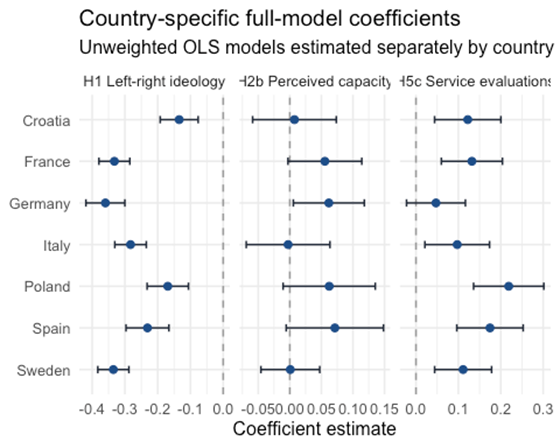
\includegraphics[width=5.2471in,height=4.19768in]{media/image4.png}~

Figure 3.~Country-specific estimates for three key predictors from the
full model.~

~

\subsection{A first look at the explanatory
patterns~}\label{a-first-look-at-the-explanatory-patterns}

Figure 4 provides a descriptive overview of the preregistered
individual-level predictors before we move to multivariable models. For
each predictor, respondents are divided into five~roughly
equal-sized~bins. The figure plots the mean value of the predictor in
each bin against the mean level of general political solidarity.~

Several patterns are already visible in the descriptive evidence.
Left-right ideology shows the clearest negative association: respondents
further to the right report lower general political solidarity.
Perceived financial capacity is positively associated with solidarity,
consistent with the idea that people are more willing to support
redistribution for others when they feel able to contribute. By
contrast, objective need and perceived risk do not show the expected
positive descriptive pattern. Objective need is almost flat, while
perceived risk is negatively associated with solidarity.~

~The strongest positive descriptive gradients appear for social trust,
institutional trust, and public-service evaluations. Respondents who
trust others, trust institutions, and evaluate public services more
positively report~substantially higher~political solidarity. This
pattern is consistent with the theoretical claim that solidarity depends
not only on individual resources or risks, but also on whether people
perceive the social and institutional environment as fair, trustworthy,
and effective.~

The binned plots are descriptive and do not adjust for country
differences or other covariates. They therefore cannot serve as
hypothesis tests. They do, however, preview the central empirical
question for the regression analysis: whether the strong associations
for trust and service evaluations remain once individual foundations and
country fixed effects are included, and whether the unexpected
descriptive patterns for resources, need, and risk persist in the full
models.~

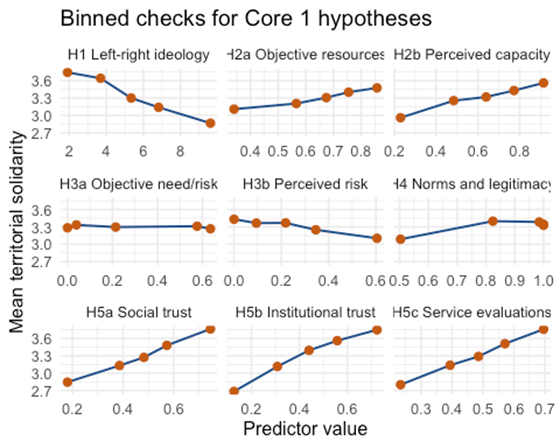
\includegraphics[width=5.83333in,height=4.66667in]{media/image5.png}~

Figure 4. Descriptive associations between preregistered predictors and
territorial solidarity.~\emph{Note:~Each panel divides respondents into
five~approximately equal-sized~bins of the focal predictor. Points show
bin-level means of territorial solidarity; lines~connect~these means.
The figure is descriptive and does not adjust for country fixed effects
or respondent-level controls. Higher values of left-right
ideology~indicate~a more right-wing position; higher values of all other
predictors~indicate~more of the construct named in the panel.}~

\subsection{Pooled models: individual foundations and
legitimacy~perceptions~}\label{pooled-models-individual-foundations-and-legitimacy-perceptions}

The pooled regression analysis (Table 2) turns the descriptive patterns
into comparable model-based tests. The full model~retains~7,058
respondents, corresponding to 87.5\% of the cleaned sample, and explains
34\% of the variation in general political solidarity.~

Among the individual foundations, left-right ideology is the clearest
predictor. More right-wing respondents are~substantially
less~politically solidary than more left-wing respondents (β = -0.266,
95\% CI {[}-0.286, -0.246{]}, p \textless{} 0.001). The
resource-and-risk results are more mixed. Perceived capacity to
contribute~remains~positively associated with solidarity in the full
model (β = 0.036, p = 0.003), and objective need/risk is also positive
(β = 0.029, p = 0.008). By contrast, objective resources are close to
zero once the attitudinal predictors are included (β = 0.005, p =
0.764), and perceived risk is not statistically distinguishable from
zero (β = 0.008, p = 0.455). These results provide~strong support~for
the ideology hypothesis and weaker but still positive evidence for
perceived capacity and objective need. They do not support a simple
cost-side resource account.~

The second block of predictors captures social norms and institutional
legitimacy. Here, all estimates are positive and precisely estimated.
Social trust (β = 0.158), institutional trust (β = 0.158), and
public-service evaluations (β = 0.135) are among the strongest
predictors in the full model. Contribution norms also~remain~positively
associated with general political solidarity (β = 0.073, p \textless{}
0.001). The pooled models therefore suggest that political solidarity is
linked not only to respondents' ideological position and material
circumstances, but also to whether they see other citizens,
institutions, and public services as trustworthy, fair, and effective.~

~

\begin{longtable}[]{@{}
  >{\raggedright\arraybackslash}p{(\linewidth - 18\tabcolsep) * \real{0.2285}}
  >{\raggedright\arraybackslash}p{(\linewidth - 18\tabcolsep) * \real{0.0680}}
  >{\raggedright\arraybackslash}p{(\linewidth - 18\tabcolsep) * \real{0.1089}}
  >{\raggedright\arraybackslash}p{(\linewidth - 18\tabcolsep) * \real{0.0833}}
  >{\raggedright\arraybackslash}p{(\linewidth - 18\tabcolsep) * \real{0.0671}}
  >{\raggedright\arraybackslash}p{(\linewidth - 18\tabcolsep) * \real{0.1010}}
  >{\raggedright\arraybackslash}p{(\linewidth - 18\tabcolsep) * \real{0.0833}}
  >{\raggedright\arraybackslash}p{(\linewidth - 18\tabcolsep) * \real{0.0680}}
  >{\raggedright\arraybackslash}p{(\linewidth - 18\tabcolsep) * \real{0.1089}}
  >{\raggedright\arraybackslash}p{(\linewidth - 18\tabcolsep) * \real{0.0833}}@{}}
\toprule\noalign{}
\begin{minipage}[b]{\linewidth}\raggedright
~
\end{minipage} &
\multicolumn{3}{>{\raggedright\arraybackslash}p{(\linewidth - 18\tabcolsep) * \real{0.2601} + 4\tabcolsep}}{%
\begin{minipage}[b]{\linewidth}\raggedright
\textbf{Block A}~
\end{minipage}} &
\multicolumn{3}{>{\raggedright\arraybackslash}p{(\linewidth - 18\tabcolsep) * \real{0.2513} + 4\tabcolsep}}{%
\begin{minipage}[b]{\linewidth}\raggedright
\textbf{Block B}~
\end{minipage}} &
\multicolumn{3}{>{\raggedright\arraybackslash}p{(\linewidth - 18\tabcolsep) * \real{0.2601} + 4\tabcolsep}@{}}{%
\begin{minipage}[b]{\linewidth}\raggedright
\textbf{Full}~
\end{minipage}} \\
\midrule\noalign{}
\endhead
\bottomrule\noalign{}
\endlastfoot
\textbf{Characteristic}~ & \textbf{Beta}~ & \textbf{95\% CI}~ &
\textbf{p-value}~ & \textbf{Beta}~ & \textbf{95\% CI}~ &
\textbf{p-value}~ & \textbf{Beta}~ & \textbf{95\% CI}~ &
\textbf{p-value}~ \\
H1 Left-right ideology~ & -0.329~ & -0.350, -0.308~ &
\textbf{\textless0.001}~ & ~ & ~ & ~ & -0.266~ & -0.286, -0.246~ &
\textbf{\textless0.001}~ \\
H2a Objective resources~ & 0.063~ & 0.031, 0.094~ &
\textbf{\textless0.001}~ & ~ & ~ & ~ & 0.005~ & -0.025, 0.034~ &
0.764~ \\
H2b Perceived capacity~ & 0.108~ & 0.083, 0.133~ &
\textbf{\textless0.001}~ & ~ & ~ & ~ & 0.036~ & 0.012, 0.059~ &
\textbf{0.003}~ \\
H3a Objective need/risk~ & 0.054~ & 0.030, 0.077~ &
\textbf{\textless0.001}~ & ~ & ~ & ~ & 0.029~ & 0.008, 0.051~ &
\textbf{0.008}~ \\
H3b Perceived risk~ & -0.029~ & -0.052, -0.006~ & \textbf{0.012}~ & ~ &
~ & ~ & 0.008~ & -0.013, 0.029~ & 0.455~ \\
H3 Risk x Capacity interaction~ & 0.001~ & -0.020, 0.022~ & 0.930~ & ~ &
~ & ~ & -0.004~ & -0.023, 0.015~ & 0.681~ \\
H4 Norms and legitimacy~ & ~ & ~ & ~ & 0.083~ & 0.063, 0.104~ &
\textbf{\textless0.001}~ & 0.073~ & 0.052, 0.094~ &
\textbf{\textless0.001}~ \\
H5a Social trust~ & ~ & ~ & ~ & 0.192~ & 0.169, 0.215~ &
\textbf{\textless0.001}~ & 0.158~ & 0.135, 0.181~ &
\textbf{\textless0.001}~ \\
H5b Institutional trust~ & ~ & ~ & ~ & 0.183~ & 0.155, 0.211~ &
\textbf{\textless0.001}~ & 0.158~ & 0.129, 0.187~ &
\textbf{\textless0.001}~ \\
H5c Service evaluations~ & ~ & ~ & ~ & 0.150~ & 0.122, 0.178~ &
\textbf{\textless0.001}~ & 0.135~ & 0.107, 0.163~ &
\textbf{\textless0.001}~ \\
Abbreviation: CI = Confidence Interval~

Table 2: Regression models of general political solidarity in seven
countries with micro-level variables only & & & & & & & & & \\
\end{longtable}

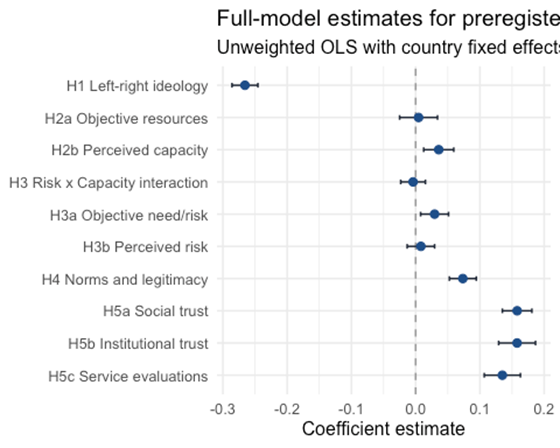
\includegraphics[width=5.83333in,height=4.66667in]{media/image6.png}~

Figure~5: Coefficient plots of full regression model for preregistered
predictors of general political solidarity.~~\emph{~}

\emph{Note:~Points show standardized OLS coefficient estimates from the
full pooled model; horizontal lines show 95\% confidence intervals. The
model includes country fixed effects and preregistered respondent-level
controls. Positive coefficients~indicate~higher general political
solidarity, measured as willingness to pay for
redistribution~benefiting~people at the municipal, national, and EU
levels. All predictors are standardized; left-right ideology is coded so
that higher values~indicate~a more right-wing position.~}

H6 is examined separately because it concerns contextual variation
rather than individual-level differences. The regional EQI analysis
decomposes public-service quality into two components. The
within-country~component~asks whether respondents living in
higher-quality NUTS2 regions are more solidaristic than respondents
living in lower-quality regions within the same country.~The
country-mean component captures cross-national differences in average
regional service quality.~These models use standard errors clustered
by~NUTS2~region.~

~The regional-context results provide little support for H6. Once the
full individual-level specification is included, the within-country EQI
coefficient is small and statistically insignificant (β = -0.010, 95\%
CI {[}-0.046, 0.025{]}, p = 0.571). The country-mean EQI coefficient is
positive and statistically significant in the simpler~models,
but~becomes statistically insignificant after trust and
service-evaluation measures are added (β = -0.031, p = 0.128 in the full
model). Relative regional income is also not robustly associated with
general political solidarity (β = 0.014, p = 0.257). Thus, the
contextual models do not show that respondents in better-performing
or~relatively richer~regions are systematically more solidaristic once
individual-level~perceptions~and controls are included.~

The pattern is nevertheless informative. The positive country-level
association between public-service quality and solidarity in the simpler
models disappears after adding trust and service evaluations. This
suggests that contextual differences in service quality may matter less
as direct regional predictors than through citizens'~perceptions~of
institutional performance, fairness, and reliability.~

\begin{longtable}[]{@{}
  >{\raggedright\arraybackslash}p{(\linewidth - 12\tabcolsep) * \real{0.1923}}
  >{\raggedright\arraybackslash}p{(\linewidth - 12\tabcolsep) * \real{0.0648}}
  >{\raggedright\arraybackslash}p{(\linewidth - 12\tabcolsep) * \real{0.0944}}
  >{\raggedright\arraybackslash}p{(\linewidth - 12\tabcolsep) * \real{0.2174}}
  >{\raggedright\arraybackslash}p{(\linewidth - 12\tabcolsep) * \real{0.0712}}
  >{\raggedright\arraybackslash}p{(\linewidth - 12\tabcolsep) * \real{0.2886}}
  >{\raggedright\arraybackslash}p{(\linewidth - 12\tabcolsep) * \real{0.0712}}@{}}
\toprule\noalign{}
\multicolumn{7}{@{}>{\raggedright\arraybackslash}p{(\linewidth - 12\tabcolsep) * \real{1.0000} + 12\tabcolsep}@{}}{%
\begin{minipage}[b]{\linewidth}\raggedright
\textbf{Table 3. Regional~public-service~quality~and general political
solidarity}~
\end{minipage}} \\
\midrule\noalign{}
\endhead
\bottomrule\noalign{}
\endlastfoot
\textbf{Model}~ & \textbf{N}~ & \textbf{NUTS2}~ & \textbf{Within-country
EQI~estimate~{[}95\% CI{]}}~ & \textbf{p-value}~ &
\textbf{Country-mean~EQI~estimate~{[}95\% CI{]}}~ & \textbf{p-value}~ \\
Baseline~ & 7,319~ & 124~ & -0.026 {[}-0.065, 0.012{]}~ & 0.183~ & 0.084
{[}0.030, 0.139{]}~ & 0.003~ \\
+~demographics~ & 7,319~ & 124~ & -0.022 {[}-0.060, 0.017{]}~ & 0.272~ &
0.075 {[}0.025, 0.126{]}~ & 0.003~ \\
+~left-right~ideology~ & 6,816~ & 123~ & 0.005 {[}-0.029, 0.039{]}~ &
0.771~ & 0.080 {[}0.028, 0.131{]}~ & 0.003~ \\
+ Block A non-ideology~ & 6,510~ & 123~ & 0.005 {[}-0.029, 0.039{]}~ &
0.779~ & 0.062 {[}0.014, 0.109{]}~ & 0.011~ \\
+~trust/service~ & 6,504~ & 123~ & -0.010 {[}-0.045, 0.026{]}~ & 0.601~
& -0.032 {[}-0.073, 0.009{]}~ & 0.131~ \\
\textbf{Full~model}~ & \textbf{6,420}~ & \textbf{123}~ & \textbf{-0.010
{[}-0.046, 0.025{]}}~ & \textbf{0.571}~ & \textbf{-0.031 {[}-0.072,
0.009{]}}~ & \textbf{0.128}~ \\
Note: Entries are standardized OLS coefficients with 95\% confidence
intervals in brackets. Standard errors are clustered by~NUTS2~region.
Models use unweighted data. EQI refers to the European Quality of
Government Index public-service quality measure.~ & & & & & & \\
\end{longtable}

~

\subsection{\texorpdfstring{Binging the micro-, meso and macro levels
together: country, region and individual mechanisms
}{Binging the micro-, meso and macro levels together: country, region and individual mechanisms }}\label{binging-the-micro--meso-and-macro-levels-together-country-region-and-individual-mechanisms}

The theoretical framework starts from a simple idea: political
solidarity is an individual attitude, but it is formed in broader
country and regional contexts. The results therefore have to be read
across levels: macro-level country differences, meso-level regional
conditions, and micro-level individual mechanisms. This cross-level
reading is useful, but it also has an important limit. The country
comparison contains seven national cases, or eight if East and West
Germany are treated separately. This is enough for a descriptive
comparison. It allows us to ask whether the country ordering fits the
theoretical expectations about welfare regimes and governance contexts.
It is not enough, however, to estimate macro-level effects with credible
statistical leverage. This is a known limitation in country-level and
multilevel comparative designs with few country units (Bryan and Jenkins
2016). The macro-level comparison in Figure 6 should therefore be read
as a descriptive benchmark: it asks whether the country ordering is
consistent with welfare-regime theory, not whether welfare regimes have
a statistically identified effect on political solidarity.

Read descriptively, the country pattern broadly fits the theory: mean
solidarity differs across welfare-state contexts in the expected
direction. To group the countries, we draw on the comparative
welfare-regime literature: Esping-Andersen's distinction between
social-democratic and conservative welfare regimes provides the classic
starting point, while Ferrera's Southern model and Fenger's
post-communist extension justify treating the Mediterranean and
Central-Eastern European cases as distinct regime contexts
(Esping-Andersen 1990; Ferrera 1996; Fenger 2007). Mean general
political solidarity, measured here by the territorial solidarity index,
ranges from 3.05 in Croatia to 3.69 in Sweden. Sweden, the only
social-democratic case in the sample, has the highest mean. Spain and
Italy, the two Mediterranean cases, also sit relatively high in the
country ordering, with an average of 3.47. The conservative and
post-communist cases are lower and more mixed: Germany and France
average 3.13 across the conservative pair, while Poland and Croatia
average 3.14 across the post-communist pair. This pattern should not be
read as a formal regime test. With so few cases, welfare institutions
cannot be separated from fiscal capacity, corruption control, political
histories, and other national differences. Still, it provides a useful
baseline for the rest of the results. Political solidarity is not
distributed evenly across national settings, and the ordering is broadly
consistent with the idea that welfare-state contexts shape how citizens
judge redistribution for others.

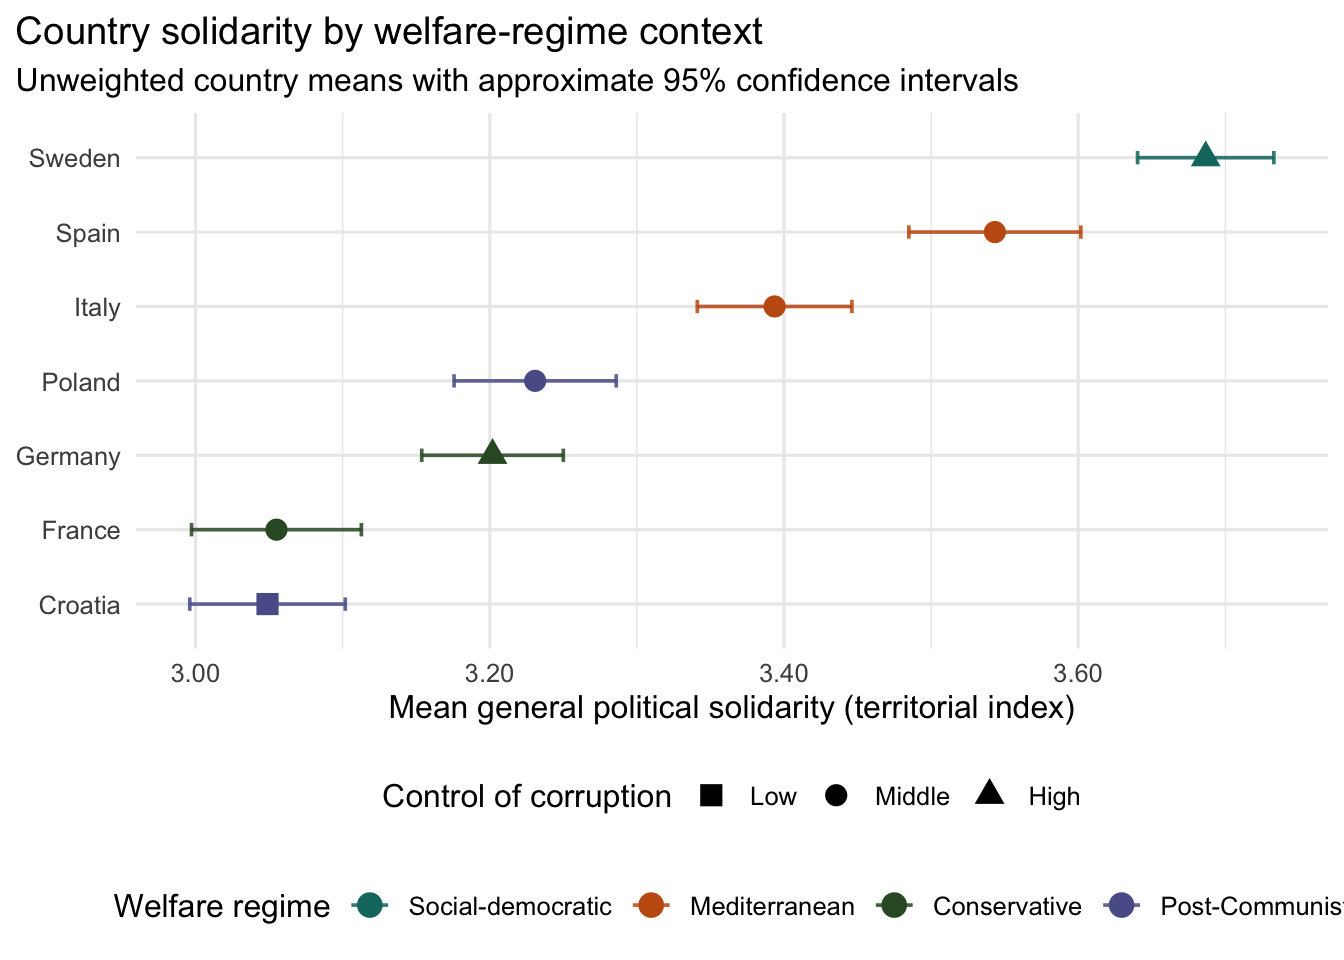
\includegraphics[width=6.26042in,height=4.46875in]{media/image7.png}Figure
6: Country means for general political solidarity by welfare-regime
context.

The plotted measure is the territorial solidarity index. The figure is
descriptive and should not be read as a macro-level test of
welfare-regime effects.

Table 4 gives the same comparison in more detail. It places the
solidarity means alongside welfare-regime classification, corruption
control, perceived governance, institutional trust, service evaluations,
and the external EQI service-quality indicator. The purpose is not to
test regime effects, but to show what kinds of country contexts
accompany the observed solidarity levels.

Table 4: Country means and contextual indicators.

\begin{longtable}[]{@{}
  >{\raggedright\arraybackslash}p{(\linewidth - 14\tabcolsep) * \real{0.1143}}
  >{\raggedright\arraybackslash}p{(\linewidth - 14\tabcolsep) * \real{0.1676}}
  >{\raggedright\arraybackslash}p{(\linewidth - 14\tabcolsep) * \real{0.1180}}
  >{\raggedleft\arraybackslash}p{(\linewidth - 14\tabcolsep) * \real{0.1107}}
  >{\raggedleft\arraybackslash}p{(\linewidth - 14\tabcolsep) * \real{0.1267}}
  >{\raggedleft\arraybackslash}p{(\linewidth - 14\tabcolsep) * \real{0.1321}}
  >{\raggedleft\arraybackslash}p{(\linewidth - 14\tabcolsep) * \real{0.1254}}
  >{\raggedleft\arraybackslash}p{(\linewidth - 14\tabcolsep) * \real{0.1051}}@{}}
\toprule\noalign{}
\endhead
\bottomrule\noalign{}
\endlastfoot
\textbf{Country} & \textbf{Welfare regime} & \textbf{Control of
corruption} & \textbf{General political solidarity} & \textbf{Perceived
governance} & \textbf{Institutional trust} & \textbf{Service
evaluations} & \textbf{Country-mean EQI service quality} \\
Sweden & Social-democratic & High & 3.687 & 0.563 & 0.557 & 0.569 &
1.254 \\
Spain & Mediterranean & Middle & 3.543 & 0.429 & 0.402 & 0.455 &
0.152 \\
Italy & Mediterranean & Middle & 3.394 & 0.424 & 0.428 & 0.419 &
-0.704 \\
Poland & Post-Communist & Middle & 3.231 & 0.457 & 0.429 & 0.485 &
-0.932 \\
Germany & Conservative & High & 3.202 & 0.496 & 0.489 & 0.502 & 0.786 \\
France & Conservative & Middle & 3.055 & 0.426 & 0.378 & 0.472 &
0.126 \\
Croatia & Post-Communist & Low & 3.049 & 0.370 & 0.318 & 0.421 &
-1.287 \\
\end{longtable}

The meso-level evidence qualifies this baseline. The regional models ask
a narrower question. Do respondents living in higher-quality NUTS2
regions, or in regions that are richer relative to their own country,
report higher political solidarity once individual predictors and
country context are taken into account? The regional indicators draw on
the European Quality of Government Index, which captures subnational
variation in corruption, impartiality, and public-service quality
(Charron, Dijkstra, and Lapuente 2014). The models do not show robust
direct regional associations. Both estimates are small and statistically
uncertain. The estimate for regional public-service quality is beta =
-0.01, 95\% CI {[}-0.046, 0.025{]}, p = 0.571. The estimate for relative
regional income is beta = 0.014, 95\% CI {[}-0.01, 0.038{]}, p = 0.257.
These estimates do not mean that regional context is irrelevant. Rather,
they suggest that the available regional indicators do not explain much
additional variation once individual attitudes, legitimacy beliefs,
social norms, and controls are included. One plausible interpretation is
that regional and country contexts matter partly by shaping the
perceptions through which citizens judge redistribution, institutions,
and other citizens (Svallfors 2013). A second, more methodological
possibility is that the linked regional indicators are too coarse, or
the within-country variation too noisy, to detect direct regional
differences in this design.

The clearest empirical pattern appears at the individual level. In the
full model, solidarity is most consistently associated with ideology,
social trust, institutional trust, service evaluations, contribution
norms, perceived capacity, and need or risk. This should not be read as
a purely individual-level explanation. Instead, it clarifies where the
present data have the most leverage. Country contexts provide different
descriptive baselines, and regional context remains theoretically
relevant, but the strongest survey evidence points to the perceptions
and orientations through which citizens evaluate the solidarity system.
In substantive terms, citizens are more willing to support
redistribution for others when the social and institutional environment
appears credible: when others are expected to contribute, institutions
are trusted, and public services are seen as fair and effective.

Figure 7 summarizes this interpretation across the three levels. The
macro layer refers to country context, the meso layer to regional
context, and the micro layer to individual attitudes, social norms, and
perceptions of state legitimacy. The overall conclusion is cautious but
still substantive: political solidarity is shaped by institutional
contexts, but in these data it is most clearly observed through
individual trust, perceived legitimacy, and evaluations of system
performance.

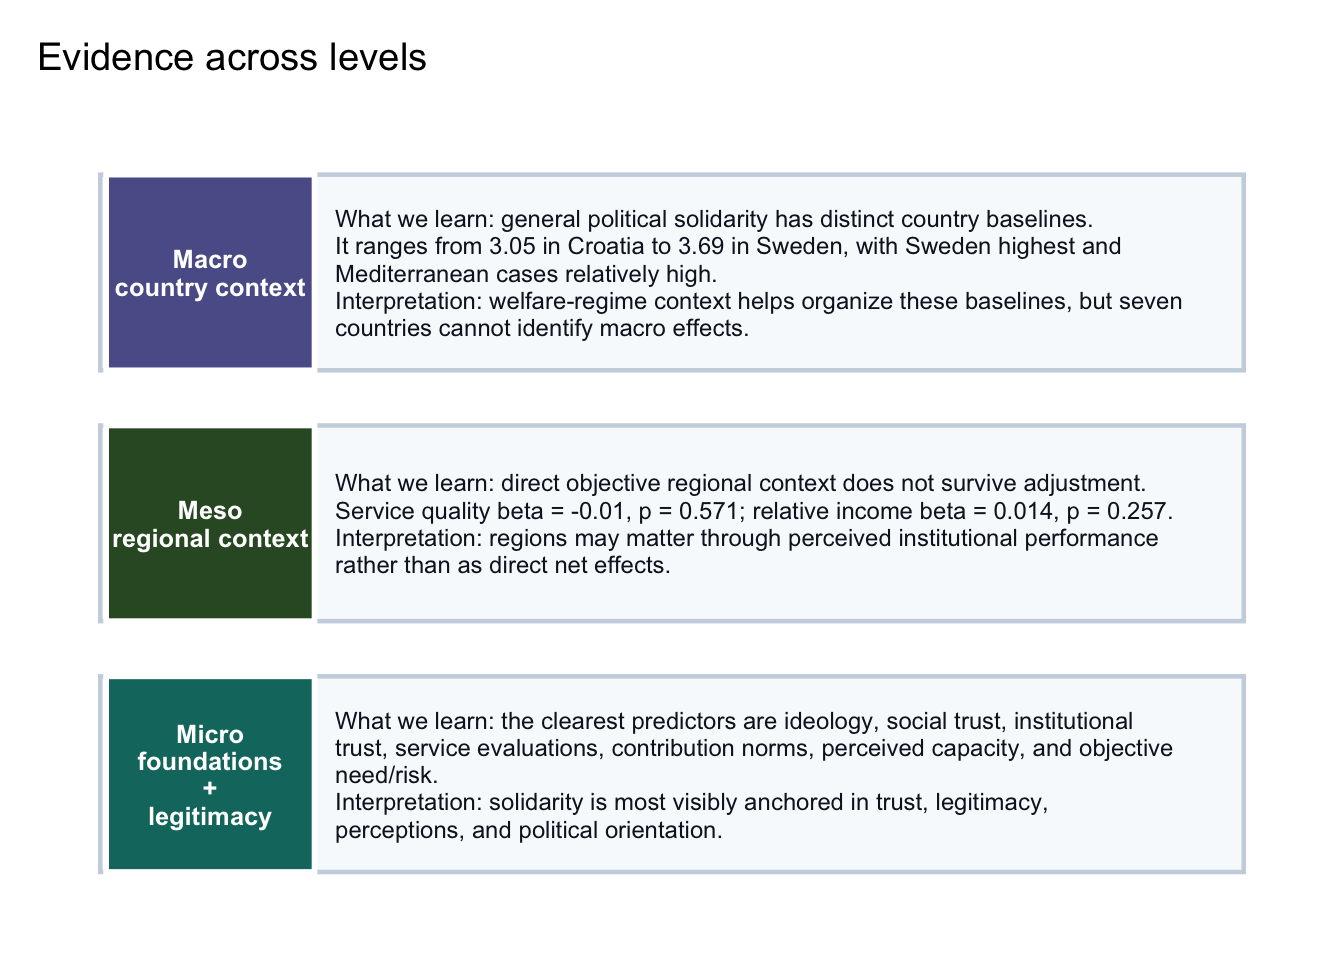
\includegraphics[width=6.26042in,height=4.46875in]{media/image8.png}Figure
7: Summary of the evidence across macro, meso, and micro levels.

\section{~Our Contributions}\label{our-contributions}

We asked what drives citizens' willingness to support costly public
redistribution for others. The results point to a~relatively
clear~pattern. Political solidarity in this seven-country sample is
strongly structured by ideology and by~perceptions~of trust,
institutional legitimacy, and public-service performance. By contrast,
objective resources, need, and regional position matter less
consistently than whether respondents see other people, institutions,
and public services as trustworthy and fair.~

~The strongest individual-level divide is ideological. Respondents on
the right are less politically solidary and draw a sharper distinction
between conventionally deserving groups and migrants. This is not
surprising, but it is substantively important. Political solidarity is
not merely a response to one's own economic position or exposure to
risk. It is also embedded in broader political orientations about
redistribution, deservingness, and the proper scope of collective
responsibility.~

At the same time, the material foundations of solidarity are more
complicated than a simple net-contributor model would suggest. We do not
find~strong evidence~that respondents with greater socioeconomic
resources are consistently less solidaristic once attitudes
and~perceptions~are~taken into account. Perceived capacity to contribute
is positively associated with solidarity, and objective need or risk
also shows some positive association. This suggests that solidarity may
be strongest not simply among those who expect to benefit, nor simply
among those who can afford to pay, but among respondents who combine a
sense of capacity with a sense that collective protection is
meaningful.~

The clearest substantive pattern concerns trust and legitimacy.
Respondents who trust other people, trust institutions, and evaluate
public services positively are more willing to support redistribution
for others. This supports the central argument of the paper: political
solidarity depends not only on distributive position, but also on
whether citizens believe that the solidarity system works. People appear
more willing to support collective redistribution when they think others
contribute~fairly,~institutions are reliable, and public services
deliver. In this sense, solidarity is not only a moral preference or a
material calculation. It is also a judgement about the credibility of
the system through which redistribution is~organised.~

The regional-context results~qualify~this argument.~We do not find
robust direct associations between regional public-service quality,
relative regional income, and general political solidary once
individual-level perceptions are included.~One interpretation is that
context matters mainly through citizens' perceptions: better-performing
institutions may shape solidarity by building trust and improving
evaluations of public services.~Another interpretation is more cautious:
the available regional indicators may be too coarse, or the
within-country variation too limited, to detect direct contextual
effects in this design. The present analysis therefore supports the
importance of perceived institutional performance more clearly than it
supports a direct regional-context effect.~

Several limitations should be kept in mind. The analysis is
cross-sectional, so the estimates should be interpreted as associations
rather than causal effects. Trust, service evaluations, and solidarity
may partly reflect common underlying dispositions, and the direction of
causality cannot be~established~here. Some preregistered measures were
only partially available in the final survey file, which narrows the
empirical coverage of the corresponding hypotheses. Finally, although
the survey allows comparison across seven country cases, it does not
cover all welfare-regime types or all forms of European regional
inequality.~

Despite these limitations, the results suggest a clear implication.
Political solidarity is unlikely to be sustained by material interest
alone. Citizens' willingness to support redistribution for others
appears to depend heavily on whether they regard the social and
institutional environment as trustworthy, fair, and effective. In
contemporary Europe, where welfare states face demographic, fiscal, and
political pressure,~maintaining~solidarity may therefore require more
than persuading citizens about need. It may also require preserving
confidence that institutions can~organise~redistribution fairly and that
others are contributing as well.~

~

\section{Appendix~}\label{appendix}

Table A.1: Operationalisation of concepts

Micro level: questionnaire-based operationalisation

\begin{longtable}[]{@{}
  >{\raggedright\arraybackslash}p{(\linewidth - 6\tabcolsep) * \real{0.0968}}
  >{\raggedright\arraybackslash}p{(\linewidth - 6\tabcolsep) * \real{0.1468}}
  >{\raggedright\arraybackslash}p{(\linewidth - 6\tabcolsep) * \real{0.3668}}
  >{\raggedright\arraybackslash}p{(\linewidth - 6\tabcolsep) * \real{0.3896}}@{}}
\toprule\noalign{}
\begin{minipage}[b]{\linewidth}\raggedright
Bucket
\end{minipage} & \begin{minipage}[b]{\linewidth}\raggedright
Concept
\end{minipage} & \begin{minipage}[b]{\linewidth}\raggedright
Questionnaire items (IDs and brief wording)
\end{minipage} & \begin{minipage}[b]{\linewidth}\raggedright
Suggested operationalisation (variables, coding, notes)
\end{minipage} \\
\midrule\noalign{}
\endhead
\bottomrule\noalign{}
\endlastfoot
Outcome & Political solidarity (willingness to support welfare for
others) & \begin{minipage}[t]{\linewidth}\raggedright
plsol1: Willingness to pay for public redistribution

Rows: my village, town or city.; \{Country\}.; other EU countries who do
not live in \{Country\}.\\
\strut \\
plsol2: Willingness to pay for target groups

Rows: children.; older people.; the poor.; people from other EU
countries who live in {[}country{]}.; people from countries outside the
EU who live in {[}country{]}.\\
\strut \\
scgv: Governmental Scope: Standard of Living

Rows: older people?; children?; the poor?; people from other EU
countries who live in {[}country{]}?; people from countries outside the
EU who live in {[}country{]}?\\
\strut \\
plsolfund: Preferred payment for public redistribution\strut
\end{minipage} & \begin{minipage}[t]{\linewidth}\raggedright
Primary DV from willingness-to-pay/support statements.\\
Build: general political solidarity, (\\
Variables: sol\_territ\_index (mean plsol1); sol\_group\_overall (mean
plsol2);\\
sol\_group\_deserving (children/older/poor); sol\_group\_migrants
(EU-in-country, nonEU-in-country);\\
welfare\_chauvinism = deserving minus migrants.\\
Responsibility analogues: resp\_* from scgv.\\
plsolfund is conditional.

Interacting plsol1 \& pslos2?\strut
\end{minipage} \\
A. Individual foundations (H1) & Economic ideology and egalitarian
values & \begin{minipage}[t]{\linewidth}\raggedright
leftright: Left-right self-placement\\
\strut \\
pol: Political orientation\\
Rows: a. The government should take measures to reduce differences in
income levels.; b. The less the government intervenes in the economy,
the better it is for {[}country{]}.; c. Gay men and lesbians should be
free to live their own lives as they wish.; d. A woman should be
prepared to cut down on her paid work for the sake of her family.\\
\strut \\
taxwelf: Trade-off: Tax and welfare state\\
\strut \\
soligame: Solidarity game\strut
\end{minipage} & \begin{minipage}[t]{\linewidth}\raggedright
Use left-right self-placement plus the political orientation grid.\\
Keep economic and cultural dimensions separate.\\
Variables: econ\_left\_index from pol rows a and b plus taxwelf (align
direction so higher = more pro-redistribution);\\
left\_right = leftright; solidarity\_behavior = soligame (0 to
100).\strut
\end{minipage} \\
A. Individual foundations (H2) & Objective resources (income) and
subjective status & \begin{minipage}[t]{\linewidth}\raggedright
hincome: Household income\\
hhsize: Household size\\
hincshare: Share of household income\\
slfstatus: Self-placement: status ladder\strut
\end{minipage} & \begin{minipage}[t]{\linewidth}\raggedright
Probably: Equivalize income by household size.\\
Variables: income\_equiv = income\_decile / sqrt(hhsize);
subjective\_status = slfstatus.\strut
\end{minipage} \\
A. Individual foundations (H2, ambiguous, see comments at the end of
hypotheses section) & Education & eduyrs: Education years &
\begin{minipage}[t]{\linewidth}\raggedright
Education can lower solidarity if it proxies income and insider
position,\\
but can raise solidarity via universalist values, trust, and broader
identities.\\
Treat sign as empirical. Variable: education\_years = eduyrs (test
linear and threshold forms).\strut
\end{minipage} \\
A. Individual foundations (H2/H3, ambiguous) & Labour market position
and occupational status proxy & EmploymentStatusKP: Economic activity:
type econhour: Economic activity: hours of paid work &
\begin{minipage}[t]{\linewidth}\raggedright
Instrument measures labour force status (not occupational prestige).\\
Use as proxy for status and risk exposure;\\
Variables: employed, unemployed (active/passive), outside labour force
(retired, disabled, care), work\_hours (if employed).\strut
\end{minipage} \\
A. Individual foundations (H3) & Objective need and benefit receipt &
\begin{minipage}[t]{\linewidth}\raggedright
pubpay: Receiving public payments\\
Rows: 1 Retirement pension; 2 Child, family or care allowance/benefit; 3
Unemployment benefit; 4 Disability benefit/pension; 5 Housing, rent or
heating benefit; 6 Social assistance or minimum income benefit\strut
\end{minipage} & \begin{minipage}[t]{\linewidth}\raggedright
Use benefit receipt as objective need/exposure.\\
Variables: benefit\_any; benefit\_count; benefit\_type dummies (pension,
child/care, unemployment, disability, social assistance, housing).\strut
\end{minipage} \\
A. Individual foundations (H3) & Perceived personal risk and future need
& \begin{minipage}[t]{\linewidth}\raggedright
prsk: Personal risk assessment\\
Rows: 1 not have enough money for everyday goods in your household?; 2
be out of work and be looking for new work for at least 4 weeks?; 3 be
unfit for work or your usual daily activities for at least 4 weeks?; 4
have less time for your job or your usual daily activities than you
would wish because you have to take care of a family member or
relative?\strut
\end{minipage} & \begin{minipage}[t]{\linewidth}\raggedright
Perceived likelihood of adverse events in next 6 months.\\
Variables: risk\_index; risk\_econ (money + unemployment);
risk\_health\_care (health limitation + care obligation).\strut
\end{minipage} \\
A. Individual foundations (H2b/H3c) & Perceived household economy and
financial resilience & \begin{minipage}[t]{\linewidth}\raggedright
eco: Current economic assessment: national economy\\
Rows: The situation of the {[}country adjective{]} economy; The
financial situation of your household;

fresil: Financial resilience\strut
\end{minipage} & \begin{minipage}[t]{\linewidth}\raggedright
Perceived capacity and scarcity.\\
Use for heterogeneity tests of the alternative mechanism where acute
strain may reduce solidarity.\\
Variables: econ\_eval\_household (eco household item);
financial\_resilience = fresil.\strut
\end{minipage} \\
B. Social norms and legitimacy (H4) & Perceived willingness of others to
contribute and norm climate &
\begin{minipage}[t]{\linewidth}\raggedright
rednrmdsc: Redistribution norm: descriptive {[}\\
rednrminj: Redistribution norm: injuctive {[}\\
sochelp: Helping norm: descriptive norm: Subjective social norm {[}Rows:
Cheating on tax if someone has the chance; Claiming state benefits which
someone is not entitled to\strut
\end{minipage} & \begin{minipage}[t]{\linewidth}\raggedright
Combine descriptive and injunctive norms plus tolerance of cheating (tax
and benefit abuse).\\
Variables: norms\_prosolidarity = mean(rednrmdsc, rednrminj, sochelp);\\
cheating\_tolerance = mean(norm items, reverse so higher means stronger
norm compliance).\strut
\end{minipage} \\
B. Social norms and legitimacy (H5a) & Generalised social trust and
fairness expectations & \begin{minipage}[t]{\linewidth}\raggedright
soctrst: social trust and helping norm: injuctive\\
\strut \\
percfair: Perceived fairness\\
\strut \\
perchelp: Perceived helpfulness\strut
\end{minipage} & Variable: social\_trust\_index = mean(soctrst,
percfair, perchelp). \\
B. Social norms and legitimacy (H5b) & Institutional trust and
democratic satisfaction & \begin{minipage}[t]{\linewidth}\raggedright
trst: Political trust Rows: {[}country{]}'s parliament?; the armed
forces?; the legal system?; politicians?; political parties?; public
authorities in your village, town or city?; ...\\
\strut \\
satdem: Satisfaction with democracy\strut
\end{minipage} & Variables: inst\_trust\_index = mean(trst items);
satisfaction\_democracy = satdem. \\
B. Social norms and legitimacy (H5c) & Public service satisfaction and
perceived relative performance &
\begin{minipage}[t]{\linewidth}\raggedright
pssatgen: Public service: overall satisfaction\\
pssatloc: Public service: relative satisfaction in local area\strut
\end{minipage} & Variables: service\_satisfaction = pssatgen;
service\_relative\_local = pssatloc. \\
B. Social norms and legitimacy (H5c, mechanism) & Perceived public
service quality across domains &
\begin{minipage}[t]{\linewidth}\raggedright
psq: Quality public sector\\
Rows: Public health care; Schools; Tax authority; e. Public transport;
Benefits and employment services; Public administration in my village,
town or city\strut
\end{minipage} & \begin{minipage}[t]{\linewidth}\raggedright
Variables: ps\_quality\_index = mean(psq rows);\\
optional domain sub-indices (social: healthcare + schools;
administrative: tax + benefits + local admin; transport separate).\strut
\end{minipage} \\
B. Social norms and legitimacy (H5c, mechanism) & Experience-based
fairness and efficiency of services & pse: Public service Rows: When I
use public services in {[}country{]}, I am treated fairly and with
respect.; Public services in {[}country{]} use resources efficiently and
are well-run.; If I need help from a public service in {[}country{]}, I
can expect to receive it promptly.; Public officials in {[}country{]}
act in the public interest, and do not abuse their position for personal
gain. & Variable: ps\_process\_index = mean(pse items). \\
C. Boundaries of solidarity & Deservingness criteria and conditional
solidarity & \begin{minipage}[t]{\linewidth}\raggedright
dsvr: Deservingness\\
Rows: People who are poor because of bad choices they made should be
denied social benefits and services.; People who receive social benefits
and services should be content instead of complaining.; It is not fair
that people receive social benefits or services to which they have not
contributed.; When granting social benefits and services, people like me
should get more priority.; Social benefits and services should only be
available to those who truly live in poverty.\strut
\end{minipage} & \begin{minipage}[t]{\linewidth}\raggedright
Variable: deservingness\_restrictive (code so higher means more
restrictive).\\
Use to explain group-specific solidarity and welfare chauvinism.\strut
\end{minipage} \\
C. Boundaries of solidarity & Immigration attitudes and correlates of
welfare chauvinism & \begin{minipage}[t]{\linewidth}\raggedright
immiforc: Immigration: forced migrants\\
\strut \\
immiecon: Immigration: economic migrants\\
immicullife: Cultural Life enriched by immigration\strut
\end{minipage} & Variable: immigration\_openness = combined index after
aligning direction (higher means more positive). \\
C. Boundaries of solidarity & Identity and in-group proximity; migration
background & \begin{minipage}[t]{\linewidth}\raggedright
id: Identification

Rows: 1 your village, town or city?; 2 \{COUNTRY\}?; 3 the European
Union?; 4 the world as a whole?\\
\strut \\
idminor: Self-identification: minority group {[}\\
citiz: Citizenship\\
borncntry: Born in country\\
\strut \\
yrinccntry: Year first living in country\\
\strut \\
bornfath: Father born in country\\
\strut \\
bornmoth: Mother born in country\strut
\end{minipage} & \begin{minipage}[t]{\linewidth}\raggedright
Variables: id\_local/id\_national/id\_EU/id\_world from id rows.\\
Migration background dummies from borncntry/bornfath/bornmoth;
minority\_self\_id from idminor.\strut
\end{minipage} \\
C. Boundaries of solidarity & Social networks and contact (ethnic,
political, class, age) & \begin{minipage}[t]{\linewidth}\raggedright
frndinch: Friends networks: rich\\
frndincl: Friends networks: poor\\
\strut \\
frndethn: Friends network: ethnicity\\
\strut \\
frndpol: Friends network: other politics\\
\strut \\
frndoldr: Friends networks: 10 years older\\
\strut \\
frndyngr: Friends networks: 10 years younger\strut
\end{minipage} & \begin{minipage}[t]{\linewidth}\raggedright
Use as moderators of otherness and norms.\\
Variables: contact\_ethnic, contact\_political, contact\_class,
contact\_age.\strut
\end{minipage} \\
Additional mechanism & Perceived tax burden and fairness of
contributions & \begin{minipage}[t]{\linewidth}\raggedright
txbrd: Current Tax Assessment\\
Rows: For those with high incomes among the highest-earning quarter of
people, taxes are \ldots; For those with middle incomes, taxes are
\ldots; For those with low incomes among the lowest-earning quarter of
people, taxes are \ldots{}\strut
\end{minipage} & Variables: perceived\_progressivity (contrast high vs
low) and tax\_burden\_index. \\
Controls & Political engagement, wellbeing, household composition,
contextual perceptions & \begin{minipage}[t]{\linewidth}\raggedright
polint: Political interest\\
\strut \\
poldisfam: Political discussions: family and friends\\
\strut \\
poldiscol: Political discussions: work colleagues\\
\strut \\
votetrnt: Recalled turnout national parliamentary election\\
\strut \\
voteprspopen: Prospective vote choice: country of interview {[}Single
Answer \& Open End{]}\\
\strut \\
lifesat: Life satisfaction\\
\strut \\
lnly: Loneliness

Rows: 1 you lack companionship?; 2 left out?; 3 isolated from others?\\
\strut \\
partner: Partnership\\
\strut \\
livtogr: Living Together\\
\strut \\
Hhchldu18: Household number children aged \textless18\\
\strut \\
crisoc: Crisis perception of country\textquotesingle s society\\
\strut \\
euintgr: European integration attitude

Age: age

Gndr: gender\strut
\end{minipage} & \begin{minipage}[t]{\linewidth}\raggedright
Use as controls and for robustness/heterogeneity tests.\\
Discussion\_frequency = mean(poldisfam, poldiscol).\\
Loneliness\_index = mean(lnly rows).\\
Perceived societal crisis (crisoc) can help probe the strain
mechanism.\strut
\end{minipage} \\
\end{longtable}

Table A. 2: Meso and macro level: external indicators (linked to micro
perceptions)

\begin{longtable}[]{@{}
  >{\raggedright\arraybackslash}p{(\linewidth - 6\tabcolsep) * \real{0.1407}}
  >{\raggedright\arraybackslash}p{(\linewidth - 6\tabcolsep) * \real{0.1156}}
  >{\raggedright\arraybackslash}p{(\linewidth - 6\tabcolsep) * \real{0.3540}}
  >{\raggedright\arraybackslash}p{(\linewidth - 6\tabcolsep) * \real{0.3896}}@{}}
\toprule\noalign{}
\begin{minipage}[b]{\linewidth}\raggedright
Level
\end{minipage} & \begin{minipage}[b]{\linewidth}\raggedright
Concept
\end{minipage} & \begin{minipage}[b]{\linewidth}\raggedright
External indicator (outside questionnaire)
\end{minipage} & \begin{minipage}[b]{\linewidth}\raggedright
Linked micro perception/mediator
\end{minipage} \\
\midrule\noalign{}
\endhead
\bottomrule\noalign{}
\endlastfoot
Region (meso) & Quality of governance (impartiality, quality, low
corruption) & QoG EU Regional Dataset (NUTS2) pillars or aggregate;
optional national WGI equivalents for robustness. & pse, psq, pssatgen,
trst \\
Region (meso) & Regional prosperity and fiscal capacity & Regional GDP
per capita (PPS) and fiscal capacity proxies; OR Regional government
revenue per capita; OR purchasing power standards per capita & eco,
fresil, txbrd \\
Region (meso) & Regional unemployment and labour market risk & Regional
unemployment rate; & prsk, EmploymentStatusKP \\
Region (meso) & Relative regional position within country & Rank or
z-score of regional indicators within country; or: deviation from
national GDPpC & pssatloc, id \\
Country (macro) & Welfare state universalism and regime type & Regime
typologies or quantitative universalism measures. & Cross-level
interactions with income and risk; taxwelf as attitudinal context \\
Country (macro) & Fiscal capacity & Government revenue per capita or
revenue-to-GDP (Eurostat/OECD). & eco, txbrd; fresil and slfstatus \\
Country (macro) & Inter-regional inequality & Variance of regional GDP
per capita and unemployment within country (ratio or Gini). & pssatloc;
welfare chauvinism contrasts \\
\end{longtable}

A.4 Imputation Summary~

Income is the only variable with~substantial~missingness. Overall, 902
income values are imputed, corresponding to 11.2\% of the sample. Other
variables have minor missingness and are imputed using simple
country-level mean or~mode~rules.~

\emph{Table A.3: Country-level summary of income imputation.~}

\begin{longtable}[]{@{}
  >{\raggedright\arraybackslash}p{(\linewidth - 8\tabcolsep) * \real{0.1172}}
  >{\raggedright\arraybackslash}p{(\linewidth - 8\tabcolsep) * \real{0.2001}}
  >{\raggedright\arraybackslash}p{(\linewidth - 8\tabcolsep) * \real{0.2374}}
  >{\raggedright\arraybackslash}p{(\linewidth - 8\tabcolsep) * \real{0.2699}}
  >{\raggedright\arraybackslash}p{(\linewidth - 8\tabcolsep) * \real{0.1754}}@{}}
\toprule\noalign{}
\begin{minipage}[b]{\linewidth}\raggedright
country~
\end{minipage} & \begin{minipage}[b]{\linewidth}\raggedright
Observed income~
\end{minipage} & \begin{minipage}[b]{\linewidth}\raggedright
Regression imputed~
\end{minipage} & \begin{minipage}[b]{\linewidth}\raggedright
Country-mean fallback~
\end{minipage} & \begin{minipage}[b]{\linewidth}\raggedright
Total imputed~
\end{minipage} \\
\midrule\noalign{}
\endhead
\bottomrule\noalign{}
\endlastfoot
Croatia~ & 88.9~ & 0.0~ & 11.1~ & 11.1~ \\
France~ & 90.9~ & 4.0~ & 5.1~ & 9.1~ \\
Germany~ & 88.6~ & 4.7~ & 6.8~ & 11.4~ \\
Italy~ & 85.9~ & 5.0~ & 9.0~ & 14.1~ \\
Poland~ & 85.8~ & 5.6~ & 8.7~ & 14.2~ \\
Spain~ & 88.8~ & 4.6~ & 6.6~ & 11.2~ \\
Sweden~ & 93.0~ & 2.9~ & 4.2~ & 7.0~ \\
\end{longtable}

4.5 Missingness~And~Retention~

\emph{Table A.4 Missingness in the variables used in the main model.~}

\begin{longtable}[]{@{}
  >{\raggedright\arraybackslash}p{(\linewidth - 8\tabcolsep) * \real{0.3148}}
  >{\raggedright\arraybackslash}p{(\linewidth - 8\tabcolsep) * \real{0.3214}}
  >{\raggedright\arraybackslash}p{(\linewidth - 8\tabcolsep) * \real{0.0884}}
  >{\raggedright\arraybackslash}p{(\linewidth - 8\tabcolsep) * \real{0.1272}}
  >{\raggedright\arraybackslash}p{(\linewidth - 8\tabcolsep) * \real{0.1482}}@{}}
\toprule\noalign{}
\begin{minipage}[b]{\linewidth}\raggedright
variable~
\end{minipage} & \begin{minipage}[b]{\linewidth}\raggedright
meaning~
\end{minipage} & \begin{minipage}[b]{\linewidth}\raggedright
n\_total~
\end{minipage} & \begin{minipage}[b]{\linewidth}\raggedright
n\_missing~
\end{minipage} & \begin{minipage}[b]{\linewidth}\raggedright
pct\_missing~
\end{minipage} \\
\midrule\noalign{}
\endhead
\bottomrule\noalign{}
\endlastfoot
left\_right\_ideology~ & Left-right self-placement, where lower values
are left and higher values are right~ & 8066~ & 576~ & 7.1~ \\
perceived\_risk\_index~ & Perceived risk of future need or deterioration
index~ & 8066~ & 346~ & 4.3~ \\
norms\_legitimacy\_index~ & Norms and perceived contribution index;
partial~Hauptfeld~version uses tax morale and welfare fraud norms~ &
8066~ & 181~ & 2.2~ \\
perceived\_capacity\_index~ & Perceived personal capacity to contribute
index~ & 8066~ & 94~ & 1.2~ \\
institutional\_trust\_index~ & Institutional trust index;
partial~Hauptfeld~version excludes politicians and parties~ & 8066~ &
36~ & 0.4~ \\
objective\_need\_index~ & Objective exposure to social need/risk index~
& 8066~ & 8~ & 0.1~ \\
solidarity\_territorial~ & Territorial solidarity index: willingness to
pay for redistribution at municipal, country, and EU levels~ & 8066~ &
0~ & 0.0~ \\
objective\_resources\_index~ & Objective socioeconomic resources index~
& 8066~ & 0~ & 0.0~ \\
social\_trust\_index~ & Generalized social trust index~ & 8066~ & 0~ &
0.0~ \\
service\_quality\_index~ & Public-service satisfaction, quality,
fairness, efficiency, helpfulness, and integrity index~ & 8066~ & 0~ &
0.0~ \\
income\_equiv~ & Household income equivalized by square-root~household
size~ & 8066~ & 0~ & 0.0~ \\
age~ & Respondent age~ & 8066~ & 0~ & 0.0~ \\
gender\_binary~ & Gender indicator: 0 male, 1 female~ & 8066~ & 0~ &
0.0~ \\
education\_level~ & Highest education level~ & 8066~ & 0~ & 0.0~ \\
migrant\_background~ & Respondent born outside country of interview~ &
8066~ & 0~ & 0.0~ \\
hincome\_imputed~ & Indicator for household income deciles imputed by
country-specific regression or fallback mean~ & 8066~ & 0~ & 0.0~ \\
\end{longtable}

The unweighted full model~retains~7058 of 8066 respondents after
listwise deletion (87.5\%).~

\end{document}
